\chapter{Introduction}
\section{Introduction}
Living in the petabyte era, we are drowning in information but starved for knowledge \cite{naisbitt1984megatrends}. Given the explosive growth of rich data from information sources, challenging difficulties of information extraction have surfaced \cite{bigdata2011}. Data mining is the process of discovering interesting and useful patterns and relationships in large volumes of data \cite{Datamini0:online}. The goal of data mining is to extract information from a data set and transform it into  functionality to solve a defined problem. While data volumes proliferate, the knowledge it creates has not kept pace \cite{bigdata2011}. Conventional data analysis methods cannot be applied effectively to data mining as it involves tremendous amounts of data with high dimensionality and complexity. Artificial Intelligence methods such as Neural Networks (NN) applied to data mining has become an increasingly important field as it has demonstrated its effectiveness over traditional data analysis techniques. The Deep Neural Networks process involves refining a representative model iteratively where a large amount of data is used to train the model and the results are validated and tested continuously. However, as the problems we are trying to model become more complex (as are real-world applications), neural networks become deeper where it is difficult to interpret why an object is classified a particular way. Furthermore, it is also difficult to validate whether the model is a true representation where the essence of the problem has been captured because of how many layers and nodes are needed in order to model the problem. 

\section{Motivation}

Since the Learning Classifier System (LCS) was developed by John Holland in the 1970s \cite{Holl75}, their capabilities for rule induction in data mining have ignited renewed interest in this area. LCSs have been chosen as the Machine Learning (ML) technique to apply to data mining as they output human-readable rules which can be interpreted. There have been a number of investigations on the architecture, where XCS, a popular implementation of LCS, have been the first to report both accurate and maximally generalised classifications \cite{bernado2003accuracy}. 

[does not flow here]
 Machine Learning techniques such as Deep Neural Networks (DNNs) have proven to be state-of-the-art in performance on problems that significantly outperform other solutions in multiple domains \cite{lecun2015deep}. However, NNs contain human cognitive bias and are heuristic. This may lead to errors made in the processes within the system. With deep learning, there are many configurations which are prone to human bias such as the filters applied to each convolution and the assignment of weights on the parameters and nodes \cite{Cognitiv47}.

DNNs are difficult to interpret where learned high-level features cannot be extracted and transferred into different domains. Discriminative DNN models have shown to be easily fooled where they classify many unrecognisable images with near certainty as belonging to a recognised class \cite{nguyen2015deep}. This demonstrates that there are differences between the way DNNs and humans recognise objects and raises questions about the generalisation capacities of DNNs. If we regard two handwritten digits in Figure \ref{fig:similar5} as vectors of pixel values and compare these values, they are very different. This is the process and the level at which a Convolutional Neural Network (CNN) would operate (Refer to Section \ref{subsubsec:cnn}). However, regarded as shapes, the two images appear similar to a human observer \cite{belongie2002shape}. As an input of an LCS are abstract features rather than pixels, it is less sensitive to image variations, where the angle, lighting and pose of objects in the images make training CNN difficult. 

\begin{figure}[H]
	\begin{center}
		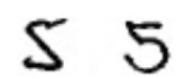
\includegraphics[width=50mm, scale=0.5]{similar5.png}
		\caption{Examples of two handwritten digit extracted from \cite{mnist}. In terms of pixel-to-pixel comparisons, these two images are different. As a human, the shapes appear similar where humans can recognise the images as fives.}
		\label{fig:similar5}
	\end{center}
\end{figure} 

Therefore, LCSs can analyse the components of an object, see the "bigger picture" and deduce knowledge which we can transfer to similar domains. For example, LCSs could be used to observe that four circular wheels are a component of a car. We can then use the learnt knowledge of the representation of a car and apply it to another object such as trucks and buses. LCSs have the ability to construct features, which will simplify the search space and therefore improve performance. This is beneficial as redundancy, irrelevancy and complexity are all problems in data mining currently. In recent years, LCSs have been optimised to solve large data mining problems. The Pittsburgh-style LCS that seeks to optimise the whole classifier, and the Michigan-style that optimise responsive rule sets \cite{brownlee2011clever} (See Section ref for more). Scalability and the ability to deal with large datasets has been a key feature when refining LCS implementations such as BioHEL (see section ref) BioHEL is designed to handle with large-scale bioinformatic datasets. These systems are suitable for large scale domains, making it possible to solve very large and complex real life problems in a suitable timeframe.

There are drawbacks in LCSs such as the solution space can be overwhelmed by too much data. The LCS solution is unhelpful with low-level inputs. Deep learning networks such as CNNs have an advantage of being able to handle large input data which contain low-level data such as pixels. Therefore, feature selection and feature construction methods will be utilised to reduce the number of features, rid of redundant and irrelevant features and find epistatic relationships between features \cite{urbanowicz2017introduction}(See Section \ref{subsubsec:fsfc}).

 TODO: low level transfer learning in CNN

\section{Aim}

The purpose of the project is to apply the concept of LCSs to Data Mining. This is to determine whether high-level representations of learnt features can be transferred to improve existing systems in order to solve new problems. The success of the project is evaluated using criteria such as accuracy, fitness and the solution's generality. Currently, an overwhelming amount of data is generated and applied to data mining systems. 

[rewrite and put somewhere else]

The system explored by this project aims to reduce the number of features by using feature selection methods, improve decision boundaries, the region of a problem space in which the output label of a classifier is ambiguous [ref] by utilising feature construction methods and provide a more compact solution than baseline solutions. 

[rewrite and put somewhere else]

Features gathered with feature selection and feature construction methods will be used in conjunction with an LCS. The produced compacted code fragments (CFs), representations of rules linking high-order "abstracted" information about input variables \cite{urbanowicz2017introduction}, can then be used to solve computer vision classification problems. In addition to this, CFs can be used as building blocks of knowledge from small problems to improve learning in problems of larger scale or similar domains \cite{urbanowicz2017introduction}. 

\section{Objectives} \label{subsec:obj}
The problems in the project can be broken down into 3 main objectives. The objectives are achieved when the criteria defined is met.


\begin{enumerate}
	\item  The goal is to create methods for extracting and integrating features from layers in a DNN as input features to a LCS to determine if this will enhance the performance on solving classification problems compared to raw features selected by the LCS. The performance will be evaluated on standard data mining benchmark datasets and will be measured on criteria such as accuracy, fitness and the solution\textquotesingle s generality (see Section \ref{sec:eval} for definitions). This will be achieved when these sub-objectives are completed:
	
	\begin{enumerate}
		\item Evaluate the performance of a LCS on benchmark datasets such as Breast Cancer Wisconsin \cite{wisconsinbreast} and Zoo Data Set \cite{zoodata}. Refer to Section \ref{subsec:datasets} for the explanations of why these datasets are used. Evaluation will be measured on criteria such as accuracy.
		\item Create a bespoke image shape dataset. The dataset will contain simple shapes without confounding variables which introduce ambiguity and distraction. Using existing image datasets such as imagenet \cite{imagenet} will increase the complexity of analysing whether the features extracted will convey a rich meaning. The dataset will be evaluated on a CNN for shape classification where evaluation is measured on the accuracy of the training and test sets.
		\item Evaluate whether features extracted from the CNN can be reused by evaluating on our benchmark datasets as well as external benchmarks such as MNIST to determine whether the features extracted convey a rich meaning.
		
	\end{enumerate}
	
	\item  The goal is to apply methods for feature selection with feature construction on LCSs where features are selected by a LCS and then constructed manually. The performance will be evaluated on standard data mining benchmark datasets and will be measured on criteria such as accuracy, fitness and the solution\textquotesingle s generality. This is to be achieved by mid-August 2018 and will be achieved when these sub-objectives are completed:
	\begin{enumerate}
		\item Create bespoke image datasets with more complex combinations of shapes such as cups where the data set is building on the dataset from the first objective.
		
		\item Construct embedded, filter or wrapper feature selection methods. These feature selection methods are defined as methods which embed the selection within the basic induction algorithm, methods which use feature selection to filter features passed to induction, and methods that treat feature selection as a wrapper around the induction process \cite{blum1997selection}.
		
		\item Evaluate these methods against the raw feature benchmarks. Evaluation will be measured on accuracy, fitness and the solution\textquotesingle s generality. 
		
	\end{enumerate}
	
	\item The goal is to implement methods for feature construction based on code fragments constructed by the LCS applied to autonomous computer vision classification problems, where the performance will be evaluated on standard data mining benchmark datasets and will be measured on criteria such as accuracy, fitness and the solution\textquotesingle s generality. This is to be achieved by the end of September 2018 and will be achieved when these sub-objectives are completed:
	\begin{enumerate}
		\item Construct feature construction methods which will further improve the accuracy, fitness or the solution\textquotesingle s generality. Feature construction methods can be used to learn more precise decision boundaries.
		
		\item Source image datasets relating to real world images and situations such as imagenet \cite{imagenet}.
	
		\item Evaluate the classifier system with feature selection and feature construction using measurement criteria such as accuracy, fitness and the solution\textquotesingle s generality.
		
	\end{enumerate}
	
\end{enumerate}
\chapter{Background}
\section{Technologies Used}
The technologies in this project include:
\begin{itemize}
\item OpenCV-Python (cv2) Library: a library of Python bindings designed to solve computer vision problems, used to preprocess images such as reading, resizing, filters such as canny and low-pass. 
\item Tensorflow/Keras Python Library: Keras is a high-level API to build and train deep learning models. used by the Mask RCNN implementation [ref]
\item Bioinformatics-oriented Hierarchical Evolutionary Learning (BioHel): BioHEL is an evolutionary learning system designed to handle with large-scale bioinformatic datasets. BioHEL is strongly influenced by the GAssist Pittsburgh LCS
\item MNIST handwritten digit dataset: has a training set of 60,000 examples, and a test set of 10,000 examples  that is commonly used for training and benchmarking various image processing systems.
\end{itemize}

\section{Related Work}
Computer vision is a field which has emerged from mathematics and computer science coupled with the psychology of perception and the neurosciences \cite{hartley2003multiple}. Many computer vision techniques have drawn inspirations from biological patterns to form algorithms such as CNNs.  From the beginning of cognitive Artificial Intelligence where Deep CNNs were popularised by Hinton  \cite{krizhevsky2012imagenet}, deep learning techniques have made huge progress in the field of computer vision and image recognition. The Conference and Workshop on Neural Information Processing Systems (NIPS) is a Machine Learning and computational neuroscience conference held every year which have involved notable publishers such LeCun \cite{lecun2015deep} who have made huge advances in DNNs. However, the performance of DNNs have rapidly outpaced our understanding of the nature of their solutions where more interpretable systems have gained interest. Biological vision still contains largely unknown factors. Unreliable naive introspection is where our visual perceptions are prone to error without the complete understanding of how vision works \cite{hartley2003multiple}. Both Deconvnets \cite{zeiler2014visualizing}, a system which visualises CNNs in an attempt to understand and improve the system, and ``Shape Matching and Object Recognition Using Shape Context'' \cite{belongie2002shape} demonstrate a need to understand the systems which we create. This project attempts to continue this work by using a LCS where code fragments can be used to convey richer knowledge which can be transferable to other domains.

[MAYBE PUT INCEPTIONISM + one PIXEL CHANGES EVERYTHING PAPER]

\section{Deep Artificial Neural Networks}
[Define here]
\subsection{Convolutional Neural Networks} \label{subsubsec:cnn}

Convolutional Neural Networks \cite{lecun2015deep} are a class of deep artificial neural networks designed to recognise visual patterns from raw data values. CNNs have been highly successful in image recognition and classification. A real world usage is face recognition on authentication systems on cellphones. However, CNNs compose of many complex connections and layers where it can be difficult to evaluate whether the learned model represents the essence of an image. A Neural Network (NN) \cite{haykin2004comprehensive} is a network composed of nodes connected by input edges and an output edge. Each node has corresponding learnable weights, which are trained using the back-propagation algorithm. These weights are real numbers expressing the importance of the input edges in relation to an output.  Back-propagation is used to calculate a gradient which is then used in the recalculation of the weights of the node. CNNs have a typical architecture, as shown in Figure \ref{fig:cnnlayers}, composed of many convolutional layers followed by a pooling layer. Fully connected layers are used at the end of the network for outputting a prediction.

\begin{figure}[H]
	\begin{center}
		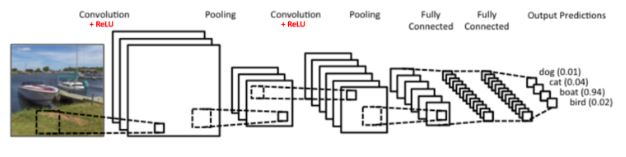
\includegraphics[width=150mm, scale=1]{cnn.JPG}
		\caption{TODO, extracted from \cite{mordvintsev2015inceptionism}}
		\label{fig:cnnlayers}
	\end{center}
\end{figure}

The primary purpose of the \textbf{\textit{convolutional}} layer is to extract features from the input image. A convolutional layer applies a convolution operation to the input and passes the outcome to the next layer. Convolutions preserve the spatial relationship between pixels by learning image features constructed by consecutively analysing small areas of an image. This is done with the convolution operation, which consists of sliding a filter, a matrix of a fixed size, over the matrix of image pixel values \cite{cnnsliding}. Different filter values contribute to different effects such as detecting edges or specific shapes in the input image. A full convolution is completed when the filter is applied to the whole matrix. The matrix formed by sliding the filter and computing the dot product between the image pixel value and the filter value is called the Feature Map.  Feature maps identify certain features of an image. Therefore, we can note that the convolutional operation's purpose is to capture locally dependent features in the original raw image. 

Additionally, a non-linearity function is applied after every convolution operation such as a Rectified Linear Unit operation (ReLU). The purpose of the non-linearity function is to introduce non-linearity into the system as most real world patterns we are trying to learn would be non-linear. Since the convolution operation involved element-wise matrix operations and is therefore a linear operation, we can account for non-linearity by introducing a non-linear function.

\textbf{\textit{Pooling layers}} is used to down sample a feature map. The result is a reduced dimensionality of the feature map but the most important information is retained. 

\textbf{\textit{Fully connected layers}} connecting every node in one layer to every node in the next layer, are used at the end of the network is used for classification of the input.

\subsection{Mask Regional CNN}
Image processing has had rapid momentum in its ability for object detection and semantic segmentation in recent years. While CNNs are very good at image classification where in some cases, can outperform humans, current image classification is less complex than true human visual understanding [ref]. This is because in classification, there is generally an image with a single object as the focus and the task is only to classify this one object. However, the real world is composed of a multitude of different overlapping objects, backgrounds and actions [ref]. Not only are humans tasked to classify multiple overlapping objects we also identify their boundaries, differences and relations to one another [ref]. 
We have seen advances driven by Fast/Faster Regional CNN and finally in 2017, Mask Regional CNN (Mask RCNN) [ref] where the architecture is shown in Figure ref. Regional CNN, an early implementation for object segmentation not only classifies multiple objects but also identifies where the objects are using bounding boxes. The bounding boxes are created using Selective Search which works by analysing the image through windows of different sizes where for each size, groups together adjacent pixels by colour or intensity to identify objects. 

However, this system is computationally expensive  where every bounding box proposal for every image needs an iteration of the CNN. the region of interest pooling techniques minimises the passes it takes to calculate the bounding boxes. This is done by sharing the iteration for an image across its subregions.  

These systems add flexibility, robustness and faster training times compared to traditional CNNs. Mask RCNN, aimed to solve instance segmentation problems, extends Faster RCNN and build upon the CNN architecture. The objective is to separate different objects in the input giving it bounding boxes, classes and masks. Mask RCNN uses a backbone which is a CNN used to extract features. There are two distinct stages of Mask RCNN. The first involves generating proposed regions of interest where an object may be present in the input image by analysing the produced feature maps and their locations on the original image. The second stage utilises another CNN which predicts the classes of the objects, refines the bounding box and generates a mask overlay based on the first proposal.


\begin{figure}[H]
	\begin{center}
		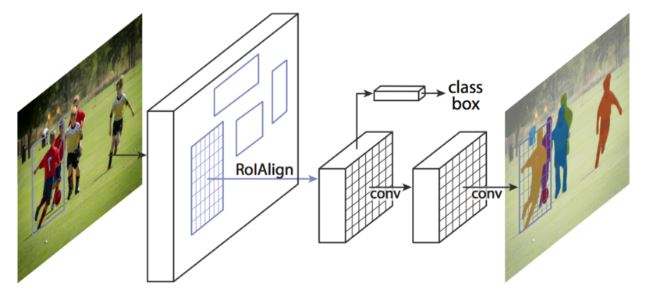
\includegraphics[width=100mm, scale=1]{maskrcnn.JPG}
		\caption{TODO, extracted from \cite{mordvintsev2015inceptionism}}
		\label{fig:cnn}
	\end{center}
\end{figure}
Deep Learning methods compose of multiple non-linear layers of filtered input which represent raw inputs as higher levels of abstraction in consecutive layers. Provided sufficient layers to perform these transformations, complex functions mapping input to output can be learned \cite{lecun2015deep}.
However, it is difficult to evaluate whether a learnt model is comparable to how a human would perceive and classify. As artificial deep learning networks are modelled from the networks of a human brain, we would expect similarities in why an input is classified. This is not the case where research has found that manipulating one pixel can the entire classification to another [ref]. Google's inceptionism also visually showcases how a CNN can fail in extracting the essence of important features. For example, a fork is a fork because of its handle and 2-4 tines. However, the shape, size, color or orientation of a fork is not important. 

Deep Learning methods such as CNNs contain many consecutive layers especially if the problem domain is complex. Therefore, it is difficult in understanding the learnt model even when dissecting each layer especially with more complex architectures like the Mask RCNN. 

[Put somewhere else]
Inceptionism \cite{szegedy2015going}, is a concept by Google engineers is used to understand and visualise how deep networks make classification decisions. Specifically, inceptionism investigates the problem of understanding the aspects of features captured in the layers of a deep model.
 \cite{mordvintsev2015inceptionism}. See section \ref{subsec:reuse} on how inceptionism was used to evaluate whether feature reuse is possible for the project.


[Put somewhere else]
Low-level pixel detection is useful for the project as a drawback of the LCS is that the induced code fragments will contain the most knowledge if the input data is represented with abstract high-level features. For example, the pixels of a car would not be useful as an input instance. However, the abstract features of four cars, windscreen and number plate would be useful. CNNs have the ability to extract abstract features from pixels by deriving information from the value and  position of pixels by sliding filters in the convolutional layer. Therefore, in the first objective, we explore the idea of whether the filters produced in the convolutional layers contain abstract features similar to the perception of what humans see.


\section{Learning Classifier System}
LCSs combine a discovery component, usually driven by Evolutionary Computation (EC) methods such as a Genetic Algorithm (GA), with a learning component \cite{urbanowicz2017introduction} such as supervised learning (refer to \ref{subsec:supervised}). The result of a LCS is a set of human readable rules which bound the classes within conditions which describe the sample space. A rule comprises a condition (specified feature states) and an action (depicting the class) which can then be interpreted as an ``IF condition, THEN action'' expression \cite{urbanowicz2017introduction}.

\subsection{Learning Cycle}

Figure \ref{fig:learningCycle} shows the learning cycle of one training instance where the main steps are described below. The structure presented is of a simple Michigan-style LCS.
\begin{figure}
	\begin{center}
		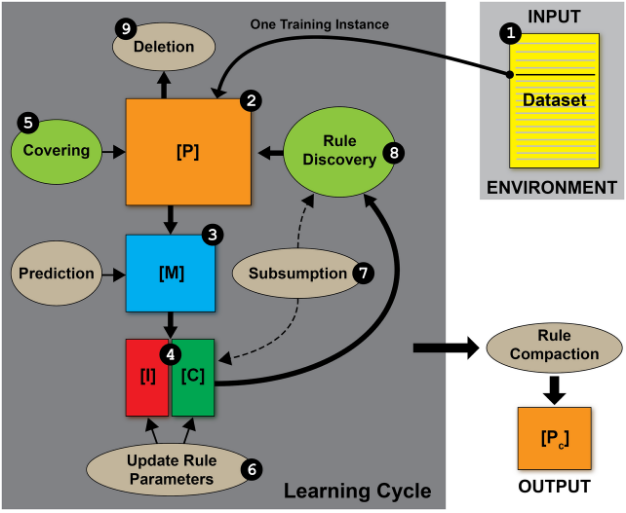
\includegraphics[width=100mm, scale=0.5]{LCScycle.png}
		\caption{LCS learning cycle, extracted from \cite{urbanowicz2017introduction}}
		\label{fig:learningCycle}
	\end{center}
\end{figure}


1.	The first step in an LCS learning cycle takes a single training instance from the environment which is the input to the population [\textit{P}].  

3. 	Matching is then performed where every rule in [\textit{P}] is now compared to the training instance to gather a set of rules which match [\textit{M}]. A matched rule occurs if all values in the rule condition is equal to the corresponding feature value in the training instance. 

4.	[\textit{M}] is then split into a correct set [\textit{C}] (rule proposes the correct action from training instance class) and an incorrect set [\textit{I}] (rule proposes the incorrect action). 

5.  Covering, typically activated in the initial learning cycle when no rules are added into  [\textit{C}] or [\textit{M}], acts as a smart population initialisation to ensure that there is at least a correct matching rule in [\textit{C}] as well as ensuring that any rule in the [\textit{P}] will match at least one training instance. Therefore, the LCS will always explore the search space in a progressive manner.

7.	Subsumption is used to remove rules which are over specific to reduce complexity and improve the efficiency of the cycle. 

8.	Rule discovery, typically using genetic algorithms selects two parents from [\textit{C}] based on their fitness. This is done using GA selection techniques such as roulette wheel selection or tournament selection. Crossover or mutation techniques are now applied to generate two offsprings. 

\subsection{LCS generality}
LCSs contain a number of components which need to be balanced in order to have a successful system. Accuracy-based systems such as XCS and UCS reward the classification based on the correctness of the predictions. Therefore, a classifier which contains rules which match all the instances is fully specific and fully accurate. However, along with accuracy and fitness, the solution\textquotesingle s generality is a criteria that is used in this project. Generality occurs when a classifier can cover more than one problem instance with a single correct action. Problems which can be classified by a single rule is called a niche \cite{urbanowicz2017introduction}. The solution obtained from the LCS should be generalised from the pressures demonstrated in Figure \ref{fig:pressureGraph} which produces an efficient, human-readable and compact solution.

Set pressure is inherent to the structure of the LCS where it is based on the principle that with generality, there is more opportunity to breed. To prevent over generality, set pressure is balanced by fitness pressure. Fitness pressure pushes the rule population towards higher specificity and increased accuracy. Rules that are not fit will not be considered for breeding and may be deleted. Rules evolve towards accurate, maximally general rules ant the generality is supported by subsumption further. However, subsumption differs from set pressure as it focusses on maximally generalising the population representation by deleting over specific rules. Mutation pressure allows the population the opportunity to get out of local maxima by providing diversification. 

\begin{figure}
	\begin{center}
		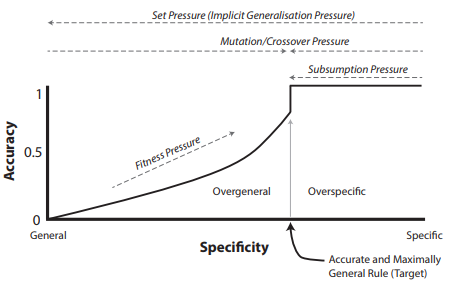
\includegraphics[width=100mm, scale=0.5]{LCSpressures.png}
		\caption{Pressures in an LCS which lead to an accurate and maximally general solution, extracted from \cite{urbanowicz2017introduction}}
		\label{fig:pressureGraph}
	\end{center}
	
\end{figure}

DNNs do not have generality pressures inherent in the structure of LCS. Introducing dropout \cite{srivastava2014dropout} and weight penalties such as L1 and L2 regularisation  \cite{srivastava2014dropout} in DNN structures prevent overfitting. However, these techniques require parameters to be set and include a certain degree of human bias. Furthermore, LCSs pressures look at the population generality based on the feature conditions and actions of a rule rather than low-level representations such as weights. 

\subsection{Architectures of LCS}

The architecture of a LCS is very flexible where it consists of components interacting with each other.  Components can be added, removed and modified to suit many problem domains. There are two main architectures, the Michigan-style architecture and the Pittsburgh-style architecture. See Section \ref{subsec:mich} for more information. 

Additionally, patterns can be found in multiple classifiers where knowledge obtained in one environment can be transferred onto a problem with a similar environment. This is possible because the features used a LCS are high level representations of the sample space compared to the raw pixel values used in Deep Learning methods \cite{zang2015learning}.

\section{Feature Selection and Feature Construction}\label{subsubsec:fsfc}

Feature selection is a common technique used to obtain a smaller set of more relevant features in order to improve the performance \cite{yu2004efficient}. This is done with some degree of cardinality reduction where the number of features are reduced to improve the quality of the feature set. Maintaining a large amount of features increases the dimensionality of the problem which can be costly in terms of complexity in time and memory as well as decreasing the quality of information. Noisy and redundant data make it more difficult to discover meaningful patterns. Other benefits of feature selection include producing a simpler, easier to interpret model where generalisations are used to reduce overfitting.

Feature construction involves transforming a given set of input features to generate a new set of more meaningful features \cite{markovitch2002feature}. Newly generated features take into account the relationships in the previous feature space. Therefore, they are more meaningful and produce more accurate classifiers and decision boundaries. 

\subsection{Low Pass Filter}
As real life objects are composed of more than basic 2D shapes, i.e. shadows, curvature and shine of the surface material, simple filters have also been applied to the image to investigate whether this would improve the performance of extracting out simple shapes. This includes using a low-pass filter to apply a blurring effect on the image. The purpose of the low-pass filter is smooth an image by reducing the amount of intensity variation between neighbouring pixels. This is particularly useful to flatten an image with shiny surface or homogenise a continuous pattern.

\subsection{Canny Algorithm}

Another filter that was investigated is the Canny filter \cite{canny1986computational}. This was used to detect edges in the image while suppressing noise as not all edges represent the outline of objects. Noise can be present in real world objects where an image with depth variations (gradients; colour variations on its surface) results in intensity changes in the object which are not edges. The canny operator will yield an image with falsely detected edges which can impact the Mask RCNN classification negatively. The purpose of extracting the outline of an image is to filter out details such as colour and texture which are not relevant.

\chapter{Design}
This project uses supervised learning to train a Michigan-style LCS and a CNN. The size and ratio of the datasets used for training has been carefully thought through. External datasets have been chosen to evaluate the classifiers.

\section{Design of experiments}
Describe the method I undertook with the experiments

\section{Supervised Training}
\label{subsec:supervised}
Supervised ML is the use of ML algorithms that utilise supplied instances to produce a model which then make predictions about future instances \cite{kotsiantis2007supervised}. The resulting classifier can then be used to assign class labels to the testing instances where instance features are known, but the value of the class label is unknown.  

In contrast, unsupervised learning is where the supplied instances are unlabelled and are generally applied to unsupervised clustering algorithms where the purpose is to discover useful classes of items \cite{jain1999data}. 
Reinforcement learning involves the input information to be provided to the learning system by the environment \cite{barto1997reinforcement}. The system must discover which actions yield the best reward by trying each action rather than being told which actions to take. 

Due to the purpose of the project being to solve classification problems, the training data will contain labelled classes making unsupervised learning technique not applicable. Reinforcement learning usually involves a more difficult process as it must explicitly explore its environment in order to determine how to act.  It is less suitable than supervised learning for the problem defined for this project as detailed training instances can be provided.

Supervised Learning is a form of inductive ML, a process where a system tries to induce general rules from a set of observed instances. The image, Figure \ref{fig:supervisedLearning} \cite{kotsiantis2007supervised}, describes the steps of supervised learning applied to a real-world problem. After the collection of data and separation of individual features and class labels, preprocessing is needed in order to remove noisy or missing feature values. There are many imputation methods which will be explored more if necessary to preprocess a specific dataset. Currently, datasets created for the purpose of validating ideas are used without the need to consider imputation. Feature selection and feature construction methods can then be used, before or during the training of the model.

\begin{figure} [H]
	\begin{center}
		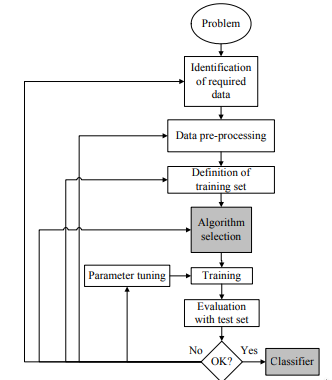
\includegraphics[width=70mm, scale=0.5]{supervisedLearning.png}
		\caption{ The process of supervised ML, extracted from \cite{kotsiantis2007supervised}}
		\label{fig:supervisedLearning}
	\end{center}
	
\end{figure}

Michigan-style LCS \label{subsec:mich}
The LCS paradigm encompasses many different problem types and learning components. There are many types of LCS which target different problem solutions. The two main variants are the Michigan-Style LCS and the Pittsburgh-Style LCS. Pittsburgh-style LCSs are closer in comparison to EC techniques as it evolves a population of solutions \cite{butz2010learning}. Michigan-style LCS involves the evolution and evaluation of rules individually \cite{butz2010learning}. Pittsburgh-style LCS suits supervised learning problem domains typical of data mining knowledge discovery from a dataset. Therefore, it runs on an offline learning environment that learns iteratively from sets of problem instances. The rule size generated is typically small and so it would be appropriate for a problem with a known solution size where the number of rules in the optimal solution is known or is small. 

In comparison, Michigan-style LCS are often run on an online learning system suitable for reinforcement learning that learns iteratively from single problem instances but can be modified for supervised offline learning systems. Michigan-style LCS is typically more flexible if the solution size is unknown or large. Therefore, the project involves exploring a Michigan approach LCS due to its flexibility. XCS is the most well-known implementation of a LCS. However, it bases its fitness on reinforcement learning methods. UCS \cite{urbanowicz2017introduction}, an adaptation of XCS for supervised learning, is accuracy and niche based and will be used in this project. 

\section{Data sets} \label{subsec:datasets}
The Wisconsin Breast Cancer \cite{wisconsinbreast} and Zoo \cite{zoodata} data sets are used in the evaluation of the baseline LCS. The Wisconsin Breast Cancer dataset has been picked in order to demonstrate that LCSs have the ability to perform when there is feature information missing in the dataset. The Zoo dataset contains imbalanced classes where the mammals class is the majority containing 41 instances compared with the amphibians class which contains 4 classes. The configured LCS was able to classify these datasets to a high degree. See Section \ref{subsec:bench} for results. 

A bespoke shapes dataset was created in order to investigate whether CNNs could produce features that can be reused by the LCS. As mentioned in my objective, an existing dataset was not used because the invariance in the images will increase the complexity of analysis unnecessarily. 

As this project currently explores the concept of supervised learning, using a training set to train instances on the learning algorithm and a test set for performance measurement is necessary. A training set is a collection of instances from which a classifier is trained. A test set is a collection of instances which is unseen by the classifier but is used for measuring the performance of the learnt classifier. By using a test set, we can validate that the classifier is generalised where overfitting has not occurred. In order of having enough instances for training whilst having a hidden set for evaluation, the well-known ratio 70:30 will be applied on the training and test sets respectively on all learning of the classifiers where this allows enough instances for the system to train on and provides enough hidden instances for validation.

Instead of using a validation set, a collection of instances used in the training to minimise overfitting, other techniques have been used during the training of the CNN. Using a dropout rate, a rate set which refers to ignoring random neurons during the training phase can also reduce overfitting. With the LCS, subsumption and the system’s pressure on generality will also reduce overfitting without the need of a validation set.

\chapter{Implementation, Evaluation and Discussion}
The first objective mentioned in Section \ref{subsec:obj} has been implemented. The goal was to create methods for extracting and integrating features from layers in a DNN as input features to the LCS. This will determine whether the higher-level features extracted could enhance the performance on solving classification problems compared to raw features selected by the LCS. 

[NOTE: ADD ERROR BARS TO ALL FINDINGS]
\section{Objective 1: Proof of Concept}
\subsection{LCS Benchmark Evaluation} \label{subsec:bench}
\begin{itemize}
	\item Evaluate the performance of a LCS on benchmark datasets such as Breast Cancer Wisconsin \cite{wisconsinbreast} and Zoo Data Set \cite{zoodata}. Refer to Section \ref{subsec:datasets} for the explanations of why these datasets are used. Evaluation will be measured on criteria such as accuracy.

\end{itemize}

For the project to succeed, there must be a good foundational understanding of how LCSs work in order to understand the specificities for the configuration of the system. The training and test set for each benchmark dataset has been split using a 70:30 split. This ratio ensures that the model has sufficient instances to learning from but also to provide a number of hidden instances to evaluate on. The dataset is also manually stratified in order to ensure a balance of all classes both the training and test set. For example, the Wisconsin Breast Cancer dataset has a 65:35 distribution of benign:malignant data. This is to ensure that the accuracy of the training will reflect in the accuracy of the test set. There are several imputation methods which can be applied to LCS. However, for easy and quick results, instances have been removed in the Breast Cancer Dataset. This is sufficient due to the distribution of the 2 classes and the number of instances being of adequate size (699 Instances).  Machine Learning classifiers are often sensitive to imbalanced training datasets as a result to the proportions of the different classes which can lead to the system favoring majority classes. However, the LCS was able to classify the Zoo data set with a reasonable outcome. Results are run 30 times and averages are presented below to ensure consistency. Evaluation is done on accuracy. See Section \ref{sec:eval} for the definition.

Results in the table below show that the trained LCS is sufficient in solving classification problems as well as having the capabilities of extracting knowledge from imbalanced domains such as the problem presented by the zoo dataset.

\begin{center}
	\begin{tabular}{ |c|c|c| } 
		\hline
		Dataset & Training Accuracy & Test Accuracy \\ 
		Zoo dataset & 100\%$\pm0.0\% $ & 97.76\% $\pm1.3\% $ \\ 
		Breast Cancer Wisconsin Dataset & 98.46\% $ \pm1.54\% $& 97.96\% $ \pm1.3\% $\\ 
		\hline
	\end{tabular}
\end{center}

\subsection{Create a data set}
\begin{itemize}
	\item Create a bespoke image shape dataset. The dataset will contain simple shapes without confounding variables which introduce ambiguity and distraction. Using existing image datasets such as imagenet \cite{imagenet} will increase the complexity of analysing whether the features extracted will convey a rich meaning. The dataset will be evaluated on a CNN for shape classification where evaluation is measured on the accuracy of the training and test sets.
	
\end{itemize}
A bespoke dataset of shapes was made in order to determine whether CNNs produced information-rich features. The dataset consists of randomly generated, black and white, class balanced, 28 X 28 basic images such as lines, circles, ellipses, squares, rectangles and triangles as seen in Figure \ref{fig:inputShapes}. It is hypothesised that shapes are the building blocks for more complex objects. Therefore, extracting the features produced by the convolutional layers may produce features which can then be used by the LCS. 
\begin{figure}[H]
	\begin{center}
		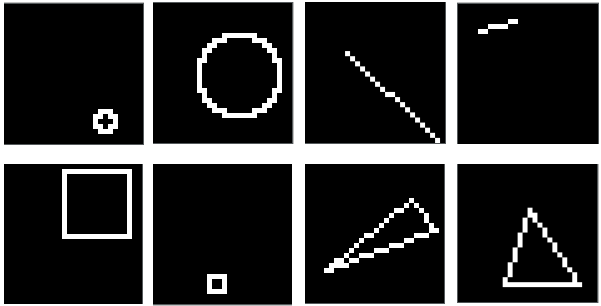
\includegraphics[width=100mm, scale=0.9]{inputShapes.png}
		\caption{Input images to CNN}
		\label{fig:inputShapes}
	\end{center}
	
\end{figure}
The structure of the CNN is shown in Figure \ref{fig:cnnStructure} where there are two convolutional layers. The model extracted had been trained on 10000 steps with 400 of each shape for training. The test set consists on 120 of each shape. Accuracy of both training and test set could reach 100\%. 

\begin{figure}[H]
	\begin{center}
		
\includegraphics[width=150mm, scale=0.9]{CNN_structure.png}
		\caption{Structure of CNN used}
		\label{fig:cnnStructure}
	\end{center}
	
\end{figure}

\subsection{Reusing features} \label{subsec:reuse}
\begin{itemize}
		\item Evaluate whether features extracted from the CNN can be reused by evaluating on our benchmark datasets as well as external benchmarks such as MNIST to determine whether the features extracted convey a rich meaning.
	
\end{itemize}

The technique of inceptionism can be used to validate that the essence of an image has been extracted. The filters produced by the training of the CNN from each convolutional layer was used as inputs by the trained CNN where predictions were outputted. The image of squares has consistently determined that straight parallel or perpendicular lines are an essential feature of squares. Using the straight parallel lines image as an input has typically resulted in the prediction of lines. This supports the idea the what humans identify as a feature of a line is similar to the CNN.  

The classifier also predicted lines significantly more than other classes. With 1280 images produced by the first convolutional layer, 509 predictions were lines (39.9\%), 279 were triangles (21.9\%), 269 (21.0\%) were squares and 223 were circles (17.4\%). This affirms the belief that shapes like triangles and squares are made up of lower-level features such as lines. Figure \ref{fig:graph_conv1} shows the composition of each class. 
\begin{figure}
	\begin{center}
		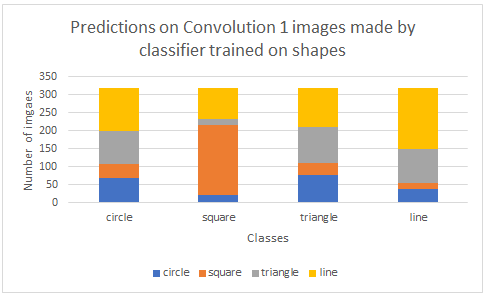
\includegraphics[width=100mm, scale=1]{graph_conv1.png}
		\caption{Prediction made in first convolutional layer}
		\label{fig:graph_conv1}
	\end{center}
	
\end{figure}

\begin{figure}
	\begin{center}
		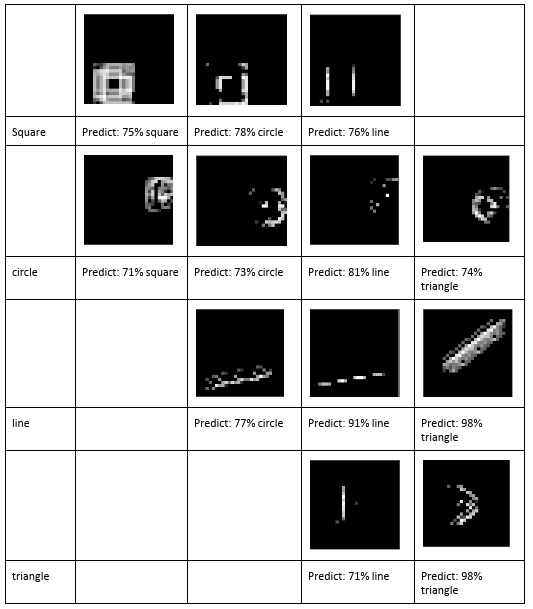
\includegraphics[width=120mm, scale=1]{conv1_pred.png}
		\caption{Example filters from the first convolutional layer}
		\label{fig:conv1_pred}
	\end{center}
	
\end{figure}

Figure \ref{fig:conv1_pred} shows examples of the images produced by the first convolution along with the predictions made by the classifier. This visualisation gives us more of an idea of the reasons behind the classification. For example, the third image shows 2 parallel lines, where the classifier classified the image as 76\% line.

Furthermore, the MNIST dataset, an image set of hand-drawn digits, was used to determine whether the features produced by the convolutional layers were able to identify the shapes produced. A sample of images from the MNIST test set was used to evaluate whether the features determined by the CNN could be interpreted by humans.  For example, a 0 would be represented by a hollow circle and an 8 would be represented by two hollowed circles stacked vertically. 

The original shapes dataset was adapted to have a white infill in order to represent the mnist data better. As even-distanced shapes such as circles and squares are less likely to occur in handwritten numbers, the dataset has further been modified to include ellipses and rectangles. During the creation of the shapes dataset, even-sided rectangles would be discarded (as they would classify as squares) and vice versa with circles and ellipses. Looking at hand drawn 0s, we would expect that a CNN which had been training on the shape dataset would classify the number as an ellipse or a circle due the roundness of edges.
Results below show the count of predicted classes [square, rectangle, circle, ellipse, line, triangle] for each MNIST class taken from a sample of 500 instances. The most popular predicted class was the ellipse. This is due to the handwritten images containing unsymmetrical curve-like edges. Unsurprisingly, lines, a pixel in width, was not predicted.  Squares were also not predicted where it is unlikely that the mnist dataset would contain any images with shape orthogonal edges. 

\begin{figure}
	\begin{center}
		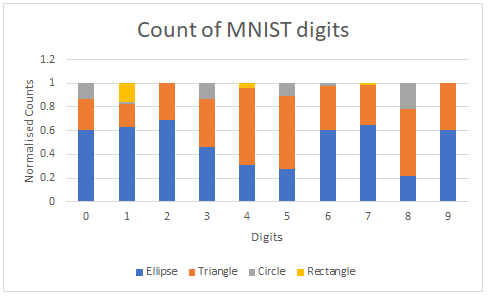
\includegraphics[width=100mm, scale=1]{graph_mnist.png}
		\caption{Count of predictions made from MNIST dataset}
		\label{fig:graph_mnist}
	\end{center}
	
\end{figure}
Figure \ref{fig:mnistseven} is an example of the classifications performed by the CNN trained on white-filled shapes. All images show handwritten sevens. The first image, classified as a rectangle, shows the 7 with very straight perpendicular lines. The second image, classified as a triangle, represents the 7 with an acute angle similar to triangles. The third image, classified as an ellipse, represents the 7 with an angle which looks more curved than the second image. 
\begin{figure}[H]
	\begin{center}
		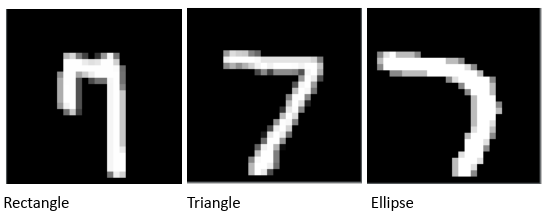
\includegraphics[width=80mm, scale=1]{mnistseven.png}
		\caption{Prediction of handwritten sevens from mnist dataset}
		\label{fig:mnistseven}
	\end{center}
	
\end{figure}
\subsection{Objective 2}
\subsubsection{1}
\begin{itemize}
	\item Create bespoke image datasets with more complex combinations of shapes such as cups where the data set is building on the dataset from the first objective.
\end{itemize}
A dataset of common, inanimate objects was created by scrapping Google images. This was done by writing a script which would return 100 Google images with Google searches such as "plain plate" or "mug". After using the scraping algorithm, the images were manually filtered for anomalies. The dataset contains 1000 images of dimension  128 X 128 is made up of a simple object such as a plate, donut, spoon, mug or fork. Of the 1000, 200 are original where transformations (rotation at 90, 180, 270 degrees and mirrored along the y-axis) are applied. Translation and scaling are transformations that are not applied to the dataset. This is because there should be efficient sizes and placements of the objects in the dataset. Images containing these features were discarded:

This is actually feature selection :O
\begin{itemize}
\item multiple objects in the image
\item bold non-continuous patterns on the object
\item background that is not monotonous/homogeneous
\item object is of similar colour and shade of background
\end{itemize}
Feature Selection Bias??? Human error
The system does not perform object segmentation where a particular object can be recognised in a cluttered situation. Therefore, multiple objects in the image would result in the Mask RCNN to identify shapes not part of the object of interest. Additionally, bold non-continuous patterns would be viewed as feature shapes being part of the object of interest. However, if the pattern is continuous, the filters (mentioned in Section ref) such as blurring the image would homogenise the pattern. 

This method of collecting images for this synthetic dataset has limitations where the images are from one source. Although Google Images provides an easily accessible, broad range of image, there is a probability of bias as the images are recommended using an algorithm. 

Refer to Appendix [ref] for a sample of the dataset 
mention different types of spoons, metal, plastic, serving etc


\section{2}
\begin{itemize}
	\item Construct embedded, filter or wrapper feature selection methods. These feature selection methods are defined as methods which embed the selection within the basic induction algorithm, methods which use feature selection to filter features passed to induction, and methods that treat feature selection as a wrapper around the induction process \cite{blum1997selection}.
\end{itemize}


\subsection{Low-pass Operator}

Python's cv2 image processing library was used to apply the low-pass filter. The procedure that I used is similar to using a mean filter, which consists of
\begin{enumerate}
\item For each pixel in image, using a 5x5 filter, look at neighbours to decide if it is representative of its surroundings.
\item For each pixel in image, replace pixels in a 5x5 filter with the mean value of its neighbours including itself
\end{enumerate}
The size of the filter results in different levels of blurring. A smaller filter size results in less of a blurring effect while a larger filter size results in a greater blurring effect as we are looking at more neighbouring pixels. A 5x5 filter size was chosen as it provided enough smoothing to reduce high intensity changes but also small enough to retain the shape of the object.

However, a limitation of applying a filter across the whole image is losing fine detail in areas which are essential in identifying an object. This is noticeable in blurring an image of a fork where the gaps in the tines are small. Therefore, when a low-pass filter if applied, the tine detailing can be lost.

\subsection{Canny Algorithm}

The canny operator was implemented by the Python cv2 library. However, I applied the low-pass filter before the canny operator to remove any noise. The process of the canny operator algorithm involves:
\begin{enumerate}
	\item Determine the intensity gradients using a edge detection operator such as Sobel, Roberts, Prewitt filter- The operator returns a value for the first derivative in the horizontal direction (Gx) and the vertical direction (Gy). The Gy mask shows interest in left-hand side columns compare to right-hand side columns where the middle columns are ignored. An edge occurs when there is a colour change and hence resulting in the intensity of pixels changing. The edge gradient can be determined by $|G|$ = $\sqrt{Gx^{2} + Gy^{2}} $. 

	\item Apply non-maximum suppression- This technique is applied to find the thickest edge in order to produce a final image with thin uniform edges.
	\item Double thresholding- To eliminate as much noise as possible, a high and low threshold is applied to remove edge pixels with weak gradient value. Edge pixels with a value greater than the high threshold is considered a strong edge pixel. Edge pixels with a value in between the two thresholds is considered a weak edge pixel. Common thresholds and the thresholds used to detect the edges in the image datasets are 100 and and 200.
	\item Edge tracking by hysteresis- This techniques is used to determine whether weak edge pixels detected in the non-maximum suppression stage is noise/colour variations or a true edge. To achieve this, the assumption that a weak edge pixel caused from real edges will be connected to a strong edge pixel whereas noise results in weak edges which are unconnected. 
	
\end{enumerate}



\paragraph{Mask RCNN Model}
loss is 0.5
The implementation of Mask RCNN [red], written on Python, Keras and Tensorflow, was based off the architecture discussed in original paper \cite{he2017mask}. A synthetic dataset created using cv2, consisting of simple shapes such as triangles, squares, circles and lines, are placed randomly on a uniform background. The colour of the shapes and background, number of shapes in the image (between 1-5), shape, size of shape and location of shapes are all randomly generated. The colour of the shapes in one image is uniform as shown in Figure \ref{fig:dataset_ex}. This is so the model is better at recognising shapes within a connected object rather than relying on edges for boundaries. 
\begin{figure}[H]
	\begin{center}
		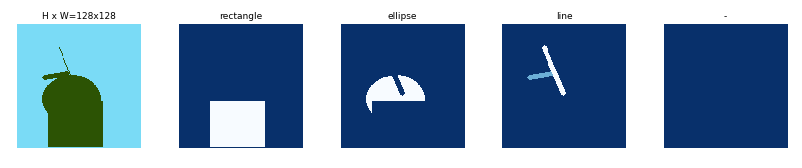
\includegraphics[width=160mm, scale=1]{maskrcnn_train.png}
		\caption{Prediction of handwritten sevens from mnist dataset}
		\label{fig:dataset_ex}
	\end{center}
	
\end{figure}


The model is then trained using a dataset of 100,000 synthetic shapes with a test dataset of 33,000 to validate and evaluate the model. [ENTER RESULT P HERE] Like many trained neural network models, weights of the nodes were initialised with a pretrained model trained on the (Common Objects in Context) COCO dataset \cite{lin2014microsoft}. This leads to a more efficient training process compared to initialising the weights to 0 or random numbers. This is because deep neural networks trained on images learn features in the first layers that are not specific to a particular dataset or task such as edges. The weight values learnt are general where they are applicable to many datasets and tasks \cite{yosinski2014transferable}.

After 50[proof needed] epochs (a single step in training), the model produced the highest p value. Training the model for more epochs results in a model overfitting on the training dataset. The purpose of the test set is to test the generality of the model to unseen instances.
 
The learning rate of the training process is 0.002. As the weights first initialised are incorrect, the back propagation algorithm is used to fix the error of the weights by transmitting the fixed error rate to lower layers (layers closer to the input) from upper layers (layers closer to output). To minimise the error of the weights, a gradient descent optimiser (such as Adam, RMSProp, Adagrad) is used (commonly known as a loss function). The learning rate is a parameter used which dictates how big of a step the optomizer is to move the weights. With a lower learning rate, the training is more reliable. However, the optimisation is more time consuming because the steps making towards minimising the loss function is small. In comparison, if the learning rate is high, the training may not converge or diverge. This is due to large weight changes where the optimiser overshoots the minimum.


\subsubsection{3}
\begin{itemize}
	\item Evaluate these methods against the raw feature benchmarks. Evaluation will be measured on accuracy, fitness and the solution\textquotesingle s generality. 
\end{itemize}

\subsection{Objective 3}
\subsubsection{1}
\begin{itemize}
	\item Construct feature construction methods which will further improve the accuracy, fitness or the solution's generality. Feature construction methods can be used to learn more precise decision boundaries.
\end{itemize}

\subsubsection{2}
\begin{itemize}
	\item Source image datasets relating to real world images and situations such as imagenet \cite{imagenet}.
\end{itemize}

\subsubsection{3}
\begin{itemize}
	\item Evaluate the classifier system with feature selection and feature construction using measurement criteria such as accuracy, fitness and the solution\textquotesingle s generality.
\end{itemize}

[TODO: WRITE UP THESE POINTS]
\begin{itemize}

	\item Bespoke dataset of 200 original input images
	\item  How I obtained the images
	  
	  - Scrapping Google images, searched for images like "plain mug"
	  
	  - Removed images that included patterns, more than 1 object i.e. multiple cups
	  
	 \item Applied filter such as sobel, low pass to see if results of individual images. Criteria of which image, original, low pass, or sobel
	 \item Process of taking output of MaskRCNN and changing it to fit input for LCS. 
	 
	 - Pick the biggest shape first and base all relationships on that
	 - Pick the shape that the MaskRCNN has outputted the biggest score.
	 \item BioHEL
	 \item CapsNet

\end{itemize}

\chapter{Evaluation}
\section{Evaluation} \label{sec:eval}
To prevent the failures relating to a waterfall model approach on the project, evaluation methods are provided for each objective mentioned in Section \ref{subsec:obj}. This methodology will validate that the findings and ideas are  meaningful at earlier stages of the project. Accuracy, fitness and the solution\textquotesingle s generality are the criteria chosen for evaluation.

For classification evaluation for LCS, accuracy is used. Accuracy is the proportion of correct classifications among all classifications \cite{urbanowicz2017introduction}. UCS is an accuracy-based LCS where accuracy is used to measure and evaluate the model whilst it is training as well as during evaluation against a test set.

Fitness (a representation of value or worth to a given rule)\cite{urbanowicz2017introduction} is another measurement to evaluate whether a specific rule is fit or not. A fitness measure relevant to supervised learning is the number of correct data classifications (action of the rule is equal to the known action from the input data) divided by the total number of times the rule has matched the input data. Fitness can be seen as the long-term accuracy of the \textit{i}th classifier.

The solution\textquotesingle s generality is also a criteria of interest as LCS can output many solution spaces. Simple solutions are prefered, containing a small set of rules which cover a large range of niches, groups of instances accurately covered by an optimal rule \cite{urbanowicz2017introduction}. 

Due to many ML techniques being stochastic, including LCSs, further tests may be beneficial in order to affirm that the results found in the project. A Student\textquotesingle s T Test compares two averages and conveys the differences from each other. This evaluation conveys whether the probability of whether the results could have occurred through chance or whether the findings convey some meaning \cite{blair1980comparison}. Therefore, the results presented will convey meaning with more certainty and confidence. An assumption of using the Student\textquotesingle s T Test is that the results will present itself as a Gaussian distribution. The classifier results will need to conducted at least 30 times in order to for the sample size to be large enough to represent a Gaussian distribution \cite{blair1980comparison}. However, if the assumption does not hold, another statistic analysis such as the Wilcoxon\textquotesingle s Ran-Sum test \cite{wilcoxon1950some} may be needed.


\chapter{Conclusion and Future Work}


